\documentclass[a4paper, landscape,11pt,exos]{nsi} % COMPILE WITH DRAFT
\usepackage{pifont}
\pagestyle{empty}

%\pb{intitulé}
%
\newcounter{pbNum}
\setcounter{pbNum}{0}
%
\newcommand{\pb}[1]
{
	\addtocounter{pbNum}{1}
	{\titlefont\color{UGLiBlue}\Large Problème\ \thepbNum\ \normalsize{#1}}\smallskip	
}

\begin{document}

\setlength\columnsep{4cm}
\begin{multicols}{2}
    \classe{\premiere spé}
    \titre{Défi de classe}
    \maketitle

    \pb{}\\
    Voici le début d'une suite.
    $$1\ ;\quad 3\ ;\quad 7\ ;\quad 15\ ;\quad 31\ ;\quad 127$$ 
    Quel est le nombre suivant ?\\
    \vfill\null
    \columnbreak
    

    \classe{\premiere spé}
    \titre{Défi de classe}
    \maketitle

    \pb{ Vrai ou faux ?}\\
    Dans un repère orthonormé, on donne :
    $$\pc{A}{-2}{3}\ ;\quad \pc{B}{5}{-1}\ ;\quad \pc{C}{2}{-4}\ ;\quad \pc{D}{-5}{0}.$$
    $ABCD$ est un parallélogramme.\\

    \newpage

    \classe{\premiere spé}
    \titre{Défi de classe}
    \maketitle

    \pb{ Vrai ou faux ?}\\
    « Tous les mathématiciens célèbres sont des hommes. »\\
    \vfill\null
    \columnbreak
    

    \classe{\premiere spé}
    \titre{Défi de classe}
    \maketitle

    \pb{}\\
    On construit des carrés. On a :\\[.5em]
    \begin{tabular}{c c c}
        
\includegraphics[width=2.5cm]{carre1} & 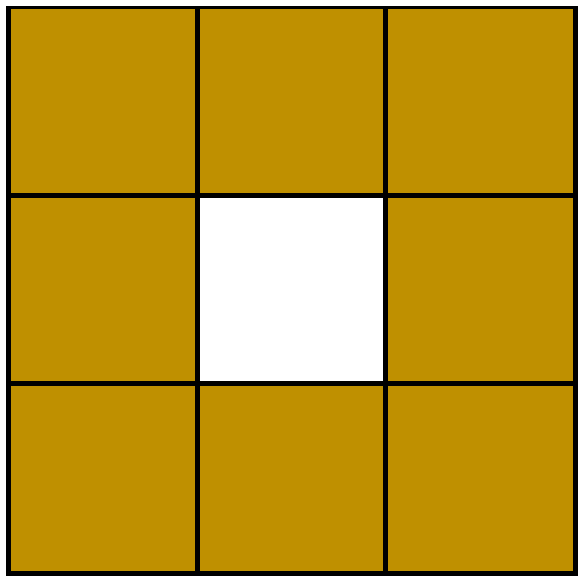
\includegraphics[width=2.5cm]{carre2} & 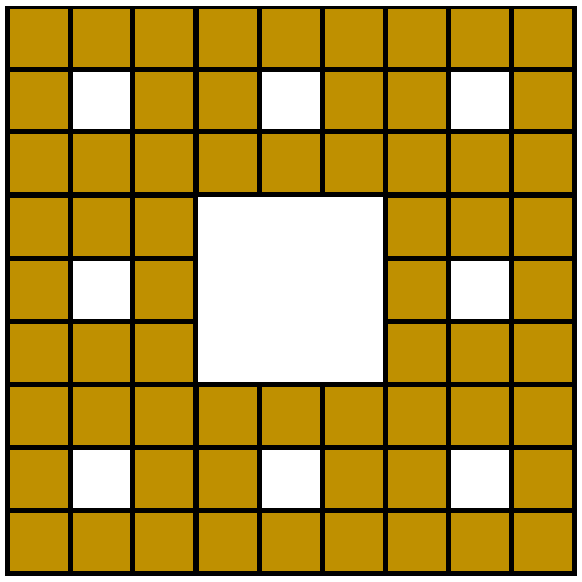
\includegraphics[width=2.5cm]{carre3}\\
        1 carré à l'épape 1 ; & 8 carrés à l'épape 2 ; & ... carrés à l'épape 3 ;\\
    \end{tabular}
    \vspace{.1cm}

    Combien a-t-on de carrés à l'étape 10 ?\\


    \newpage

    \classe{\premiere spé}
    \titre{Défi de classe}
    \maketitle
    
    \pb{}\\
    Quel est l’ensemble des solutions de l’équation $x^2-4=0$ ?\\
    \vfill\null
    \columnbreak
    

    \classe{\premiere spé}
    \titre{Défi de classe}
    \maketitle

    \pb{}\\
    $a, b$ et $c$ sont trois nombres relatifs non nuls dont le produit est négatif.\\
    $a$ est l’inverse de $c$. Quel est le signe de $b$ ?\\

    \newpage

    \classe{\premiere spé}
    \titre{Défi de classe}
    \maketitle

    \pb{ Vrai ou faux ?}\\
    « La somme des chiffres d’un nombre premier n’est jamais un multiple de 3. »\\
    \vfill\null
    \columnbreak
    

    \classe{\premiere spé}
    \titre{Défi de classe}
    \maketitle

    \dleft{5cm}
    {
    \pb{}\\
    Voici le début d'une suite :\\[.5em]
    Quel est le polygone suivant ?\\
    }
    {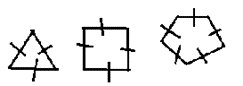
\includegraphics[width=6cm]{polynomes.png}}


    \newpage

    \classe{\premiere spé}
    \titre{Défi de classe}
    \maketitle

    \pb{ Vrai ou faux ?}\\
    « Tout nombre positif est plus grand que sa racine carrée. »\\
    \vfill\null
    \columnbreak
    

    \classe{\premiere spé}
    \titre{Défi de classe}
    \maketitle

    \pb{}\\
    IJK a un périmètre de 18 cm et ses côtés ont une longueur entière.\\
    Si IJ = 7 cm, quelle peut être la longueur de JK et KI ?\\
    Y-a-t-il plusieurs cas possibles ? Si oui, les donner tous.\\

    \newpage

    \classe{\premiere spé}
    \titre{Défi de classe}
    \maketitle

    \pb{ Vrai ou faux ?}\\
    « La somme des chiffres d’un nombre premier n’est jamais un multiple de 9. »\\
    \vfill\null
    \columnbreak

    \classe{\premiere spé}
    \titre{Défi de classe}
    \maketitle

    \pb{ Vrai ou faux ?}\\
    « Si un nombre est divisible par 6 alors son carré est divisible par 9. »\\

    \newpage

    \classe{\premiere spé}
    \titre{Défi de classe}
    \maketitle


    \pb{ Vrai ou faux ?}\\
    Dans un repère orthonormé, on donne :
    $$\pc{E}{-2}{-1}\ ;\quad \pc{F}{0}{2}\ ;\quad \pc{G}{4}{0}\ ;\quad \pc{H}{6}{3}.$$
    $EFGGH$ est un parallélogramme.\\
    \vfill\null
    \columnbreak

    \classe{\premiere spé}
    \titre{Défi de classe}
    \maketitle

    \pb{}\\
    On donne le script Python suivant :
    \begin{pyc}
        \begin{minted}{python}
n = input('Choisir un nombre entier compris entre 1 et 10)
for i in range(2) :
    if n % 2 == 0 :   # a % b donne le reste de la division euclidienne de a par b
        n = n/2
    else :
        n = 3*n+1
print(n)
        \end{minted}
    \end{pyc}

    Le programme affiche 11.\\
    Quel est le nombre qui a été choisi au départ ?\\

    \newpage

    \classe{\premiere spé}
    \titre{Défi de classe}
    \maketitle

    \pb{}\\
    Quel est l’ensemble des solutions de l’inéquation $4x-3>5x+7$ ?
    \vfill\null
    \columnbreak

    \classe{\premiere spé}
    \titre{Défi de classe}
    \maketitle

    \pb{ Vrai ou faux ?}\\
    L’aire d’un carré est proportionnelle à la longueur de son côté.
\end{multicols}







\end{document}